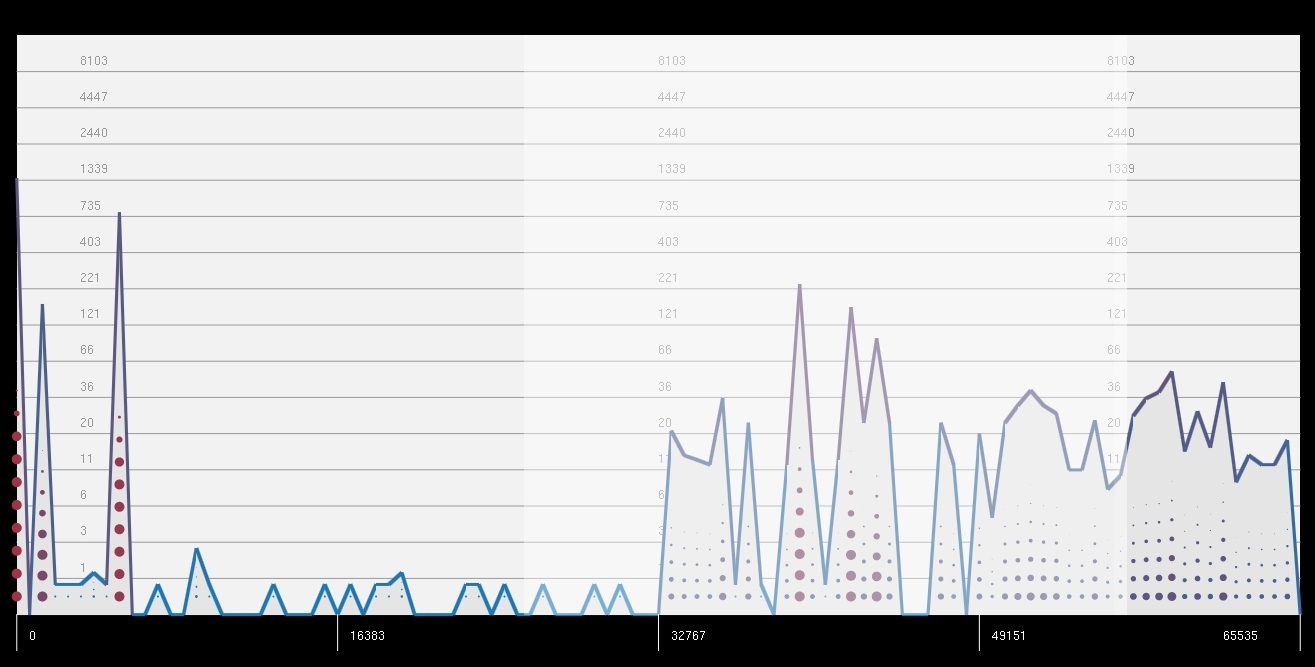
\includegraphics[width=\linewidth]{materials/distribution.jpg}

The most common need in the analysis of network traffic is to get information on the distribution of certain features of the packets. For the graph constructed here, the user selects such a feature (e.g., ports or destination IPs). A logarithmic line graph is then drawn, and (as with all visualizations in the application) updated in real time. A logarithm is applied to assist in detecting spikes.

A second layer of the visualization is presented to the user simultaneously: Circles under the line graph indicate the actual distribution (without a logarithm applied) through their area. Furthermore, all lines and circles are colour-coded to give extra signals of the volume of traffic. Red elements are under heavier load.

All these features have a single purpose: make the analyst understand what is going on, and to make obvious any anomalies.

This visualisation makes active use of the normalisers described above. It also allows the user to click-and-drag along interesting data which then automatically applies a filter to the data so that all visualizations focus on this user-selected area of interest.
